%%=============================================================================
%% Methodologie
%%=============================================================================

\chapter{De compilatie van Kotlin/Native}
\label{ch:compiler}
Kotlin is een programmeertaal die gebruik maakt van de JVM. Sinds de beslissing van JetBrains om zich ook te focussen op cross-platform development, moesten ze met een oplossing komen voor de JVM. De JVM wordt namelijk niet ondersteund op alle besturingssystemen. Zo ondersteunen bijvoorbeeld MacOS en iOS (mobile) geen JVM. JetBrains moest dus op zoek gaan naar een oplossing... de LLVM compiler. Deze compiler is een reeds bestaande compiler en is dus niet ontwikkeld in functie van Kotlin. Deze literatuurstudie is uitgevoerd aan de hand van de aosabook van LLVM, \textcite{aosa}, een zeer uitgebreide documentatie. 

\section{Wat is LLVM?}
Het LLVM-project is een verzameling modulaire en herbruikbare compiler- en toolchaintechnologieën. Het project is ontwikkeld door de LLVM developer group, waarvan Vikram Adve en Chris Lattner de originele ontwikkelaars zijn. De naam 'LLVM' zelf is geen acroniem, het is de volledige naam van het project. Ondanks de naam heeft LLVM weinig te maken met de traditionele virtuele machines.

Het LLVM-project begon als een onderzoeksproject aan de universiteit van Illinois, met als doel een compilatiestrategie aan te bieden die in staat is om zowel statische als dynamische compilatie van programmeertalen aan te bieden. Een voorbeeld van een statische taal is Java, een voorbeeld van een dynamische taal is Javascript. Zowel beide types van programmeertalen kunnen dus gecompileerd worden door LLVM.

Sinds het ontstaan van LLVM is het project uitgegroeid tot een overkoepelend project dat bestaat uit een aantal deelprojecten. Veel van deze deelprojecten worden momenteel sterk gebruikt bij commerciële en open-source projecten en zelfs in academisch onderzoek.

Enkele voorbeelden van commerciële en open-source projecten zijn:
\begin{itemize}
	\item \textbf{Vuo}, een moderne visuele programmeertaal voor multimedia ontwerpers.
	\item \textbf{Pony}, een object-georiënteerde programmeertaal.
	\item \textbf{Crack}, een programmeertaal die het gemak van de ontwikkeling van een scripttaal biedt met de uitvoering van een gecompileerde taal.
\end{itemize}

Het grote voordeel van het gebruik van LLVM is de veelzijdigheid, flexibiliteit en herbruikbaarheid. Dit wil zeggen dat het zo goed als in ieder soort project kan worden geïntegreerd. Het wordt daarom tegenwoordig gebruikt voor een groot aantal verschillende taken, dit gaande van het compileren van enkele kleine code-projecten tot het compileren van code voor massieve computers \autocite{LLVM}.

\subsection{Deelprojecten LLVM}
Enkele voorbeelden van deelprojecten van de LLVM developers group \autocite{LLVM}:
\begin{itemize}
	\item \textbf{Clang} is een LLVM native C/C++/Objective-C compiler dat als doel heeft om verbazingwekkend snelle compilaties aan te bieden. Het zorgt overigens voor nuttige fout- en waarschuwingsberichten.
	\item Het \textbf{LLDB} project bouwt verder op libraries die aangeboden worden door LLVM en Clang om te zorgen voor een native debugger.
	\item Het \textbf{libc++} en \textbf{libc++ ABI} project voorziet een krachtige implementatie van de standaard C++ bibliotheek, met ondersteuning voor C++11. 
\end{itemize}

\section{De werking van LLVM}
LLVM is dus een bibliotheek die gebruikt wordt om tussenliggende en/of machine-code te genereren en optimaliseren. Maar wat is nu de exacte werking van deze compiler? De werking van de LLVM is totaal verschillend dan die van bijvoorbeeld de JVM. Zie sectie \ref{sec:jvm} voor meer uitleg.

\subsection{De werking van een standaard compiler}
Het meest populaire ontwerp voor een statische compiler, zoals de meeste C-compilers, is het driefasenontwerp waarbij de belangrijkste componenten de \textbf{frontend}, de \textbf{optimizer} en de \textbf{backend} zijn. 

\begin{figure} [ht]
	\centering
	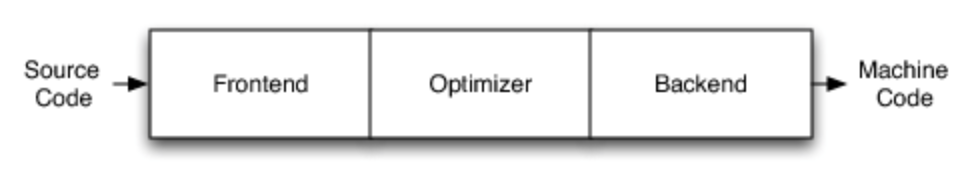
\includegraphics[width=0.95\textwidth]{img/driefasenmodel}
	\caption{Driefasenontwerp (\cite{aosa})}
	\label{fig:driefasenontwerp}
\end{figure}

\subsubsection{De frontend}
De frontend zorgt voor de analyse van de broncode. Deze heeft dus als taak om ervoor te zorgen dat geen code gecompileerd kan worden waarbij fouten aanwezig zijn. Dit gebeurt door het opstellen van een taalspecifieke abstracte syntaxboom om de syntaxcode voor te stellen. Deze syntaxboom wordt optioneel geconverteerd naar een nieuwe boom voor optimalisatie en de optimizer en de backend worden uitgevoerd aan de hand van deze boom. De JVM (Javac) is ook een implementatie van dit driefasenontwerp. Een voorbeeld van een syntaxboom is te zien in figuur \ref{fig:syntaxtree}.

\begin{figure} [ht]
	\centering
	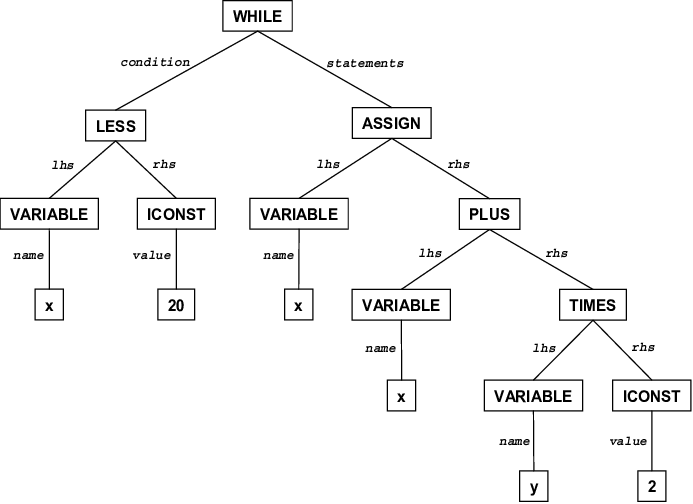
\includegraphics[width=0.95\textwidth]{img/syntaxtree.png}
	\caption{Taalspecifieke abstracte syntaxboom (\cite{ResearchGate})}
	\label{fig:syntaxtree}
\end{figure}

\subsubsection{De optimizer}
De optimizer is verantwoordelijk, zoals de naam het zelfs zegt, voor het uitvoeren van een breed gamma van transformaties om de uitvoeringstijd van de code te optimaliseren. Dit wordt gedaan door het elimineren van overtollige berekeningen, maar dit is meestal afhankelijk van de taal die gebruikt werd en de doelarchitectuur.

\subsubsection{De backend}
De backend, ook bekend als de codegenerator, gaat de code gaan mappen naar een instructieset. Naast het maken van deze instructieset is het ook verantwoordelijk om ervoor te zorgen dat deze instructieset gebruik maakt van de ongewone kenmerken van de ondersteunde architectuur. Iedere architectuur is namelijk anders en de gegenereerde instructieset moet dus afgestemd worden op de doelarchitectuur.

\subsection{Meerdere front- en backends}
Het grote voordeel van dit driefasenontwerp treedt op wanneer een compiler besluit om meerdere brontalen en architecturen te ondersteunen. Indien de optimizer een gemeenschappelijke code representatie gebruikt, dan kan een frontend geschreven worden voor elke taal die gecompileerd kan worden naar die gemeenschappelijke representatie, en een backend kan worden geschreven voor elke doelarchitectuur dat daaruit kan compileren. Door het gebruik van deze gemeenschappelijke code representatie heeft de optimizer geen kennis nodig van de doelarchitectuur. Op figuur \ref{fig:llvmdriefasen} is te zien dat door de common optimizer te gebruiken, er meerdere frontends kunnen worden geschreven en meerdere doelarchitecturen kunnen worden ondersteund.

Met dit ontwerp, indien men wenst een nieuwe brontaal te ondersteunen, moet men enkel een nieuwe frontend schrijven maar de bestaande optimizer en backend kunnen worden hergebruikt. Indien deze delen (frontend, optimizer en backend) niet waren gescheiden, zou het implementeren van een nieuwe brontaal vereisen om helemaal opnieuw te beginnen, dus een volledig nieuwe compiler te schrijven. Indien men N doelarchitecturen heeft en M brontalen, dan zou men N*M compilers hebben.

Nog een voordeel van dit ontwerp is dat deze soorten van compilers een veel bredere set van programmeurs kan tevreden stellen. Dit is minder het geval indien men slechts één brontaal en doelarchitectuur zou ondersteunen. 

\begin{figure} [ht]
	\centering
	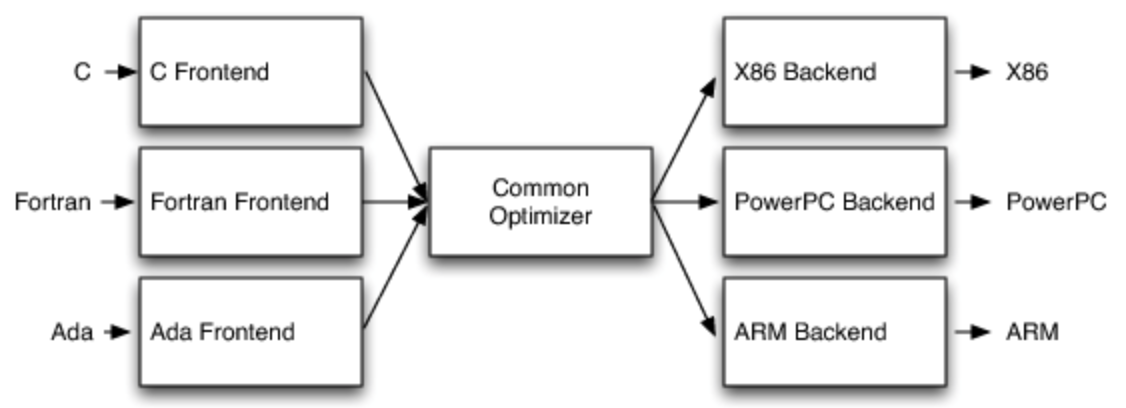
\includegraphics[width=0.95\textwidth]{img/llvmdriefasen}
	\caption{Meerdere front- en backends (\cite{aosa})}
	\label{fig:llvmdriefasen}
\end{figure}

\section{LLVM en het driefasenontwerp}
\label{sec:difference-llvm}
In een LLVM-gebaseerde compiler heeft de frontend dezelfde taak als de frontend in een normale compiler. De code wordt daarna door de frontend vertaald naar LLVM intermediate representation (IR), dit meestal door het opbouwen van een syntaxboom en deze later te converteren naar IR. De IR is eigenlijk het hart van de LLVM. Het is een low-level programmeertaal die zeer dicht aansluit bij assembly code. Deze IR heeft als taak om de code te verbeteren, waarna deze code in een soort van codegenerator wordt gestoken waarbij deze wordt omgezet naar native machinecode. 

In een korte notendop: de frontend krijgt een brontaal binnen en gaat deze taal parsen, valideren en analyseren. Hij stelt de syntaxboom op en zet deze om naar LLVM IR. De optimizer gaat de code optimaliseren en stuurt de IR code naar de backend die dient als codegenerator met als resultaat machinecode.

LLVM is dus een implementatie van het driefasenontwerp. Het grote verschil tussen een gewone implementatie van dit ontwerp en LLVM is het gebruik van de IR. Deze IR is de enige interface voor de optimizer. Dit betekent dat men enkel moet weten wat IR en wat de werking van deze IR is om een frontend te schrijven voor deze LLVM, wat het ondersteunen van nieuwe talen veel makkelijker maakt.

\begin{figure} [ht]
	\centering
	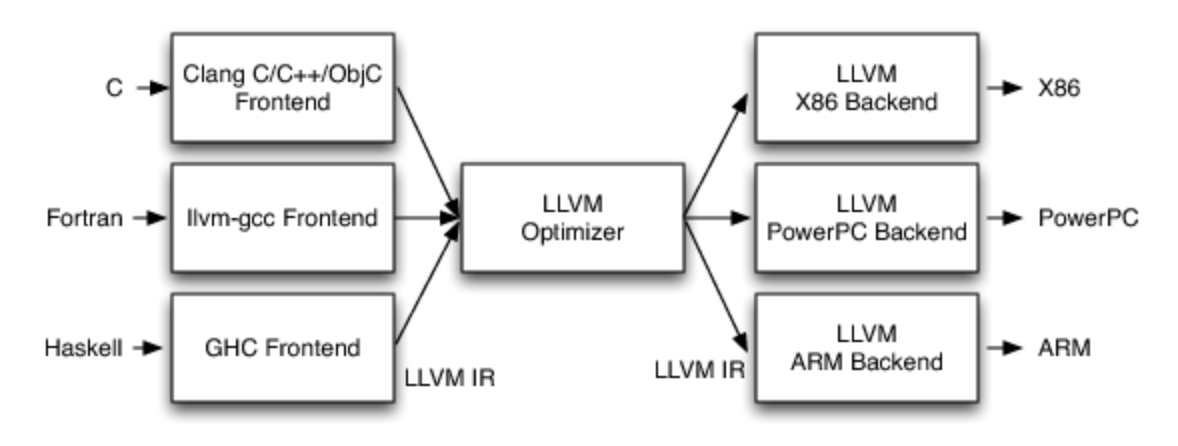
\includegraphics[width=0.95\textwidth]{img/llvmirdriefasen}
	\caption{LLVM implementatie van driefasenontwerp (\cite{aosa})}
	\label{fig:llvmirdriefasen}
\end{figure}

\section{LLVM en Kotlin/Native}
Kotlin/Native is een technologie dat Kotlin via LLVM direct compileert naar machine code. De Kotlin/Native compiler produceert zelfstandige uitvoerbare bestanden die zonder virtuele machine kunnen worden uitgevoerd. Hierdoor is het mogelijk om Kotlin te gebruiken op ieder platform of besturingssysteem.

\section{Java Virtual Machine (JVM)}
\label{sec:jvm}
De Java Virtual Machine, ook wel JVM genoemd, is een virtuele machine voor het uitvoeren van Java bytecode \autocite{TechopediaBytecode}. De JVM maakt gebruik van de Javac, de compiler die verantwoordelijk is voor het omzetten van Java-code naar bytecode. Deze bytecode is een object-georiënteerde code die gecompileerd is om op een virtuele machine te worden uitgevoerd. De code kan op elk besturingssysteem of platform, waarvoor er een JVM beschikbaar is, worden gebruikt. De virtuele machine transformeert de code, geschreven in een bepaalde programmeertaal, in machinetaal die door de CPU\footnote{Central Processing Unit} van een systeem kan worden uitgevoerd. Deze machinetaal moet geoptimaliseerd zijn voor de CPU aangezien andere platformen verschillende interpretatietechnieken kunnen gebruiken. Dit alles gebeurt at-runtime. Bij de JVM zal de bytecode meestal het resultaat zijn van de compilatie van Java-code. Echter kunnen talen zoals Scala, Clojure, Groovy en natuurlijk Kotlin (maar via de Kotlinc compiler) ook uitgevoerd worden op deze virtuele machine. De JVM heeft kennis van geheugenbeheer, optimalisatie van de uitvoering van de applicatie en garbage collection. Daarnaast begrijpt de JVM het concept van objecten en virtuele methode aanroepen. De gebruiker hoeft hierdoor geen rekening te houden met deze drie zaken. Deze virtuele machine kan ook gebruikt worden voor Kotlin. Echter zal de Javac vervangen worden door de Kotlinc compiler die geoptimaliseerd is voor Kotlin \autocite{TechopediaJVM}. 

\section{LLVM en JVM}
LLVM en JVM zijn twee aparte dingen. De JVM is, zoals te lezen in sectie \ref{sec:jvm}, een vertaler die broncode omzet naar machinetaal die door de processor van een computer onmiddelijk kan worden uitgevoerd. Het is een high-level virtuele machine aangezien deze kennis heeft van zaken zoals de garbage collection, geheugenbeheer en objecten. Bij de JVM gebeurt alles at-runtime. 

De LLVM is een low-level register gebaseerde compilatie technologie. Het neemt de LLVM IR, zie sectie \ref{sec:difference-llvm}, en gaat deze overbrengen naar native uitvoerbare bestanden voor een specifiek platform. LLVM kan tijdens het vertaalproces naar IR veel optimalisaties uitvoeren. Echter gebeurt bij de LLVM alles at-compiletime.
